\documentclass{ximera}

\begin{document}
	\author{Stitz-Zeager}
	\xmtitle{Exercises for Set Theory}{}

\mfpicnumber{1} \opengraphsfile{ExercisesforAppSetTheory} % mfpic settings added 


\label{ExercisesforAppSetTheory}

\begin{problem}
Find a verbal description for $O = \{ 2n-1 \, | \, n \in \mathbb{N}\}$    

\begin{solution}
     $O$ is the odd natural numbers.
\end{solution}

\end{problem}

\begin{problem}
Find a roster description for $X = \{ z^2 \, | \, z \in \mathbb{Z}\}$    

\begin{solution}
    $X = \{ 0, 1, 4, 9, 16, \ldots \}$
\end{solution}

\end{problem}
 
\begin{problem}
Let $A = \left\{ -3, -1.02, -\dfrac{3}{5}, 0.57, 1.\overline{23}, \sqrt{3}, 5.2020020002 \ldots, \dfrac{20}{10}, 117 \right\}$ 

\begin{enumerate}

\item  List the elements of $A$ which are natural numbers.

\begin{solution}
    $\dfrac{20}{10} = 2$ and $117$
\end{solution}

\item  List the elements of $A$ which are irrational numbers.

\begin{solution}
    $\sqrt{3}$ and $5.2020020002$
\end{solution}

\item  Find $A \cap \mathbb{Z}$

\begin{solution}
    $\left\{ -3, \dfrac{20}{10}, 117\right\}$
\end{solution}

\item  Find $A \cap \mathbb{Q}$

\begin{solution}
    $\left\{ -3, -1.02, -\dfrac{3}{5}, 0.57, 1.\overline{23},\dfrac{20}{10}, 117 \right \}$
\end{solution}

\end{enumerate}
\end{problem}

\begin{problem}
Fill in the chart below. 

\begin{center}
\begin{tabular}{|c|c|c|} \hline

Set of Real Numbers & Interval Notation &  Region on the Real Number Line  \\
\hline

& &  \\

\shortstack{$\{x\,|\,-1\leq x< 5\}$ \\ \hfill} &  &  \\ \hline

 \\

 & \shortstack{$[0,3)$ \\ \hfill} &   \\ \hline


& &  \\

 &  & 

\begin{tikzpicture}[scale=1.2]

% Horizontal axis line 
\draw (-2,0) -- (2,0);

% Filled point at (2,0)
\fill (2,0) circle (2pt);

% Open point at (-2,0)
\draw (-2,0) circle (2pt);

% Endpoint labels
\node[below] at (-2,0) {$2$};
\node[below] at (2,0) {$7$};

\end{tikzpicture}

   \\
\hline

 &  & \\
 
\shortstack{$\{x\,|\, -5 <  x \leq 0 \}$ \\ \hfill} &  & \\ \hline

 &  & \\
 
  & \shortstack{$(-3,3)$ \\ \hfill} &  \\ \hline

&  & \\
 
& & 

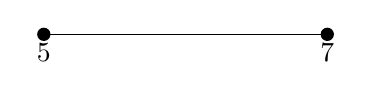
\begin{tikzpicture}[scale=1.2]

% Horizontal axis line
\draw (-1,0) -- (2,0);

% Filled point at (2,0)
\fill (2,0) circle (2pt);

% Filled point at (-1,0)
\fill (-1,0) circle (2pt);

% Endpoint labels
\node[below] at (-1,0) {$5$};
\node[below] at (2,0) {$7$};

\end{tikzpicture}
   \\
\hline

&  & \\

\shortstack{$\{x\,| \, x \leq 3 \}$ \\ \hfill} &  &  \\ \hline

 &  & \\
 
& \shortstack{$(-\infty, 9)$ \\ \hfill} &  \\ \hline

 &  & \\

 &  &  

\begin{tikzpicture}[scale=1.2]

% Horizontal axis line 
\draw (-2,0) -> (2,0);

% Filled point at (-2,0)
\fill (-2,0) circle (2pt);

% Endpoint labels
\node[below] at (-2,0) {$4$};
\node at (2,0) {$>$};

\end{tikzpicture}
   \\
\hline

 &  & \\
 
 
\shortstack{$\{x\,| \, x \geq  -3 \}$ \\ \hfill} & &    \\ \hline

\end{tabular}

\end{center}

\end{problem}

\begin{question}
In Exercises \ref{findunionintfirst} - \ref{findunionintlast}, find the indicated intersection or union and simplify if possible.  Express your answers in interval notation.    

\begin{problem}\label{findunionintfirst}
$(-1,5] \cap [0,8)$ 

\begin{solution}
    $[0,5]$
\end{solution}

\end{problem}

\begin{problem}
$(-1,1) \cup [0,6]$

\begin{solution}
    $(-1,6]$
\end{solution}
\end{problem}

\begin{problem}
$(-\infty,4]\cap (0,\infty)$

\begin{solution}
    $(0,4]$
\end{solution}
\end{problem}

\begin{problem}
$(-\infty,0) \cap [1,5]$

\begin{solution}
    $\emptyset$
\end{solution}
\end{problem}

\begin{problem}
$(-\infty, 0) \cup [1,5]$

\begin{solution}
    $(-\infty,0) \cup [1,5]$
\end{solution}
\end{problem}

\begin{problem}\label{findunionintlast}
$(-\infty, 5] \cap [5,8)$ 

\begin{solution}
     $\left\{ 5\right\}$
\end{solution}
\end{problem}

\end{question}

\begin{question}
In Exercises \ref{writeintervalfirst} - \ref{writeintervallast}, write the set using interval notation.   

\begin{problem}\label{writeintervalfirst}
$\{x\,|\, x \neq 5 \}$ 

\begin{solution}
    $(-\infty, 5) \cup (5, \infty)$
\end{solution}
\end{problem}

\begin{problem}
$\{x\,|\, x \neq -1 \}$

\begin{solution}
    $(-\infty, -1) \cup (-1, \infty)$
\end{solution}
\end{problem}

\begin{problem}
$\{x\,|\, x \neq -3,\, 4 \}$

\begin{solution}
     $(-\infty, -3) \cup (-3, 4)\cup (4, \infty)$
\end{solution}
\end{problem}

\begin{problem}
$\{x\,|\, x \neq 0, \, 2 \}$

\begin{solution}
    $(-\infty, 0) \cup (0, 2)\cup (2, \infty)$
\end{solution}
\end{problem}

\begin{problem}
$\{x\,|\, x \neq 2, \, -2 \}$

\begin{solution}
    $(-\infty, -2) \cup (-2, 2)\cup (2, \infty)$
\end{solution}
\end{problem}

\begin{problem}
$\{x\,|\, x \neq 0,\, \pm 4 \}$

\begin{solution}
    $(-\infty, -4) \cup (-4, 0) \cup (0, 4) \cup (4, \infty)$
\end{solution}
\end{problem}

\begin{problem}
$\{x\,|\, x \leq -1 \, \text{or} \, x \geq 1 \}$

\begin{solution}
    $(-\infty, -1] \cup [1, \infty)$
\end{solution}
\end{problem}

\begin{problem}
$\{x\,|\, x < 3 \, \text{and} \, x \geq 2 \}$

\begin{solution}
    $[2, 3)$
\end{solution}
\end{problem}

\begin{problem}
$\{x\,|\, x \leq -3 \, \text{or} \, x > 0 \}$

\begin{solution}
    $(-\infty, -3] \cup (0, \infty)$
\end{solution}
\end{problem}

\begin{problem}
  $\{x\,|\, x \leq 2 \, \text{and} \, x > 3 \}$  

  \begin{solution}
      $\emptyset$
  \end{solution}
\end{problem}

\begin{problem}
$\{x\,|\, x > 2 \, \text{or} \, x = \pm 1 \}$  

\begin{solution}
    $\{-1\} \cup \{1\} \cup (2, \infty)$
\end{solution}
\end{problem}

\begin{problem}\label{writeintervallast}
$\{x\,|\,  3 < x < 13 \, \text{and} \, x \neq 4 \}$

\begin{solution}
     $(3,4) \cup (4, 13)$
\end{solution}
\end{problem}

\end{question}

\begin{question}
For Exercises \ref{shadevennfirst} - \ref{shadevennlast}, use the blank Venn Diagram below with $A$, $B$, and $C$ in it as a guide to help you shade the following sets.

\begin{center}
\begin{tikzpicture}[scale=2]

% Circles
\draw (0.5,-0.875) circle (1);   % Circle C
\draw (0,0) circle (1);          % Circle A
\draw (0.875,0) circle (1);      % Circle B

% Labels
\node at (-1.25,0) {$A$};
\node at (2.125,0) {$B$};
\node at (0.5,-2.125) {$C$};
\node at (2.375,1.5) {$U$};

% Rectangle
\draw (-1.75,-2.625) rectangle (2.625,1.75);

\end{tikzpicture}

\end{center}

\begin{problem}\label{shadevennfirst}
$A \cup C$
\end{problem}

\begin{problem}
$B \cap C$
\end{problem}

\begin{problem}
$(A \cup B) \cup C$
\end{problem}

\begin{problem}
$(A \cap B) \cap C$ 
\end{problem}

\begin{problem}\label{intoverunion}
$A \cap (B \cup C)$
\end{problem}

\begin{problem}\label{shadevennlast}
$(A \cap B) \cup (A \cap C)$
\end{problem}

\end{question}


\begin{problem}
Explain how your answers to problems \ref{intoverunion} and \ref{shadevennlast} show $A \cap (B \cup C) = (A \cap B) \cup (A \cap C)$.  Phrased differently, this shows `intersection \textit{distributes} over union.'  Discuss with your classmates if  `union' distributes over `intersection.'  Use a Venn Diagram to support your answer.
\end{problem}

\begin{problem}
Show that $A \subseteq B$ if and only if $A \cup B = B$.
\end{problem}

\begin{problem}
Let $A = \{1,3,5,7,9\}, B = \{2,4,6,8,10\}, C = \{1,6,9\}$ and $D = \{2,7,10\}$.  Draw one Venn Diagram that shows all four of these sets.  What sort of difficulties do you encounter?  
\end{problem}



\end{document}
